%%%%%%%%%%%%%%%%%%%%%%%%%%%%%%%%%%%%%%%%%%%%%%%%%%%%%%%%%%%%%%%%%%%%%%%%%%%%%%%%
%2345678901234567890123456789012345678901234567890123456789012345678901234567890
%        1         2         3         4         5         6         7         8
% THESIS CHAPTER


\chapter{Vision: Methods \& Results}
\label{chap:vision}
\ifpdf
    \graphicspath{{Vision/Figures/PNG/}{Vision/Figures/PDF/}{Vision/Figures/}}
\else
    \graphicspath{{Vision/Figures/EPS/}{Vision/Figures/}}
\fi

\begin{figure}[H]
	\centering
	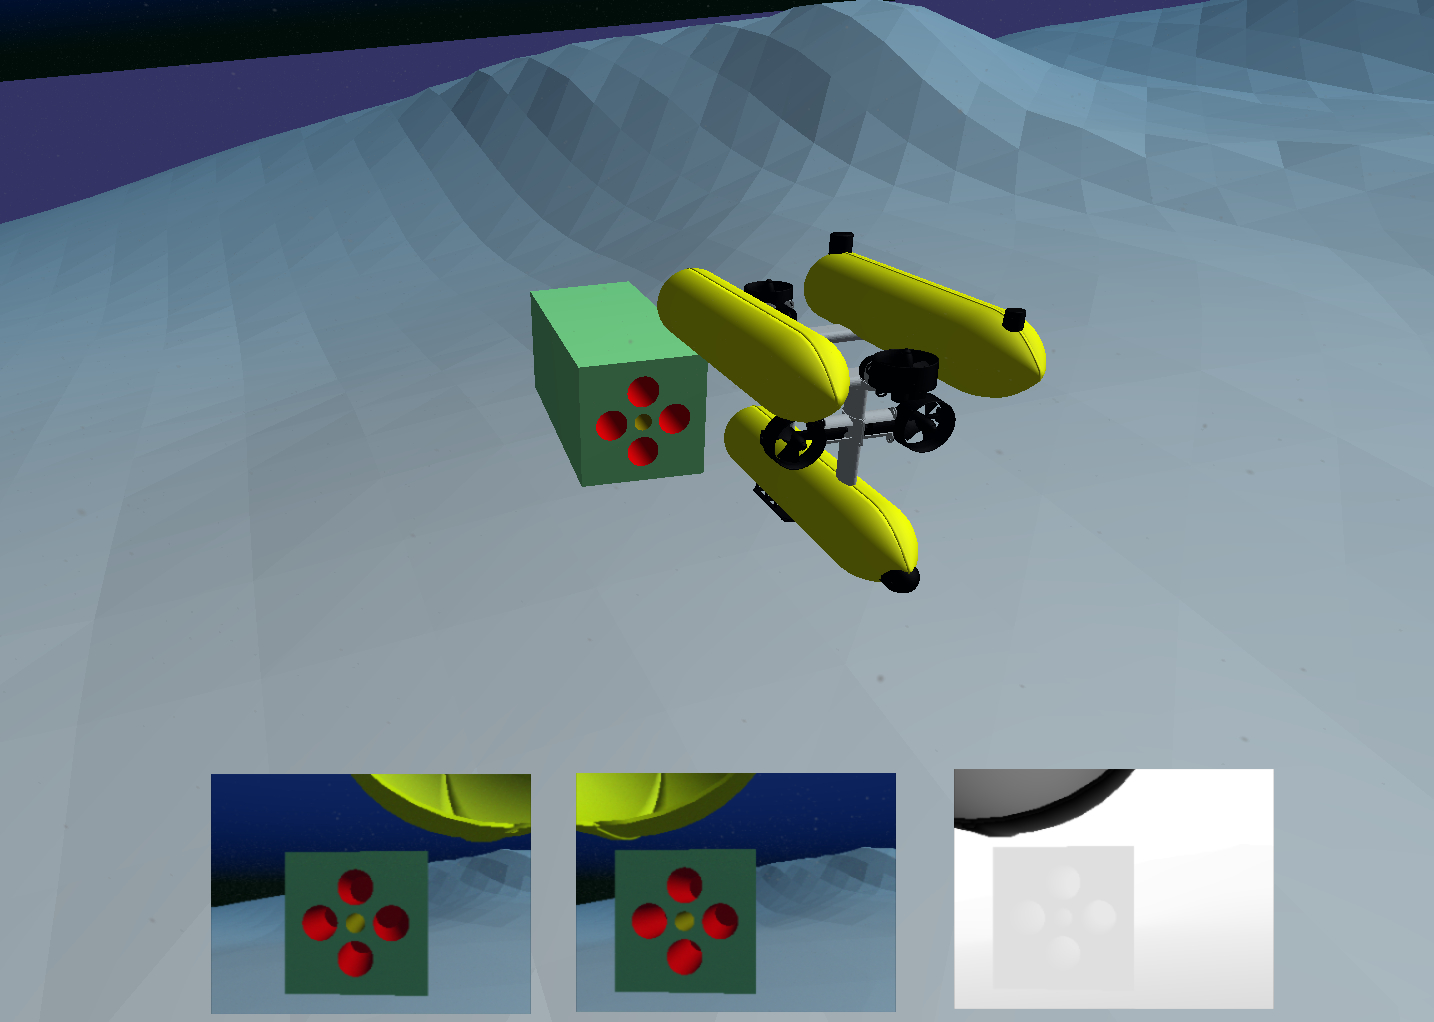
\includegraphics[width=12.0cm]{Vision_uwsim.jpeg}
	\caption[The Vision Robot watching the hole]{The \textit{vision} Robot watching the hole. The hole is in the centre of the cuboid. The red holes are only present to help vision algorithms. Below, what the right and left camera are seeing. Note that also a depth left image is provided, but the left RGB camera and the depth camera are not used together.}
	\label{fig:vision-uwsim}
\end{figure}


Before the twin robots can approach the hole, its position must be know, at least roughly. In this chapter, the pose estimation of it is discussed.\\
In the considered scenario, a third robot is present. Its duty is exclusively to \textit{detect} \& to \textit{track} the hole. In the simulation, another \href{https://cirs.udg.edu/auvs-technology/auvs/girona-500-auv/}{Girona 500 AUV} is used for this job, without the arm. Is evident that, in real scenario, a littler and more efficient robot should be used for the vision, see that no manipulation task are needed. In fact, in the original TWINBOT [\cite{TWINBOT2019}] simulation, a smaller \href{https://bluerobotics.com/product-category/rov/bluerov2/}{BlueROV} is present, as can be seen in (TODO) %todo ref figura original twinbot.
However, in this case, another Girona 500 is used to not deal with another robot model.\\
The \textit{vision} robot is equipped with two identical cameras which point in front of it. They are used as:
\begin{itemize}
	\item Two distinct cameras, independent one of the other.
	\item As stereo cameras, thus exploiting stereo vision algorithms.
	\item As RGB-D camera, i.e., a stereo vision couple where the left one is a RGB camera and the right one a Depth camera.  
\end{itemize} 
\vspace{10px}
The job is done into two phases: \textit{Detection} (section \ref{sec:visDetect}) and \textit{Tracking} \mbox{(section \ref{sec:visTracking}).} 

\section{Assumptions}
\label{sec:visioAssumption} %cited by method chapter in assumption section
For the sake of simplicity, some assumptions are made:
\begin{itemize}
	\item Known \textit{intrinsic} camera parameters. These parameters are used by algorithms to take into account how the single camera see the scene. The (known) distortion is zero.
	\item Known \textit{extrinsic} camera parameters, i.e. the position and orientation of cameras (respect the vehicle), and thus the relative pose (the transformation matrix) from one camera to the other (needed for stereo vision algorithm).
	\item No external disturbances for the images, such as light reflections underwater or bad visibility.
	\item Hole model known. This means that dimensions of the cuboid which contains the hole are known. Further explanation about this are given successively in section \ref{sec:visTracking}.
	\item A "friendly" cuboid structure of the hole. The front face is coloured and additional holes are present, as can be seen in fig. \ref{fig:vision-uwsim}. This help both the \textit{detection} phase and the \textit{tracking} phase.
\end{itemize}
About the robot, other assumption are:
\begin{itemize}
	\item the pose of the vehicle respect the inertial frame is known. (TODO?AS explained?? se si linka sez). This permits to know the estimation of the pose of the hole respect the inertial frame, to directly send the robot which are carrying the peg.
	\item The initial position of the robot is such that it is facing the front face of the hole. It must be noticed that methods explained in the next sections can be adapted to relax this hypothesis. For example, the robot could turn around z-axis until the hole is detected. (TODO?? %todo maybe far vedere sti good result? )
	 Also, good results are obtained when the robot not exactly face directly the cuboid, but, for example, it is on its side, looking at front face and a side one.
	\item Once the robot has tracked the hole and the pose sent to the twin robots, it must go away to not interfere with the insertion phase. This is done through keyboard (as a ROV) but it is not difficult to improve the code to let him go away autonomously. It must be noticed that, thanks to the \textit{tracking} algorithms, if the robot moves (because it is commanded to do so, or for water currents) the pose estimation is still good. 
\end{itemize}

\section{Tools}
\label{sec:visionTools}
To deal with the pose estimation, some external tools are used. In this section they are listed.

\begin{itemize}


	\item \href{https://opencv.org/}{\textbf{OpenCV}} (Open Source Computer Vision Library) [\cite{opencv}],  an open-source BSD-licensed library that includes several hundreds of computer vision algorithms. It is used mostly for the detection part, even if some of its functionalities are used also by ViSP (for example for keypoint tracking).
	
	\item \href{https://visp.inria.fr/}{\textbf{ViSP}} (Visual Servoing Platform) [\cite{visp}], another open source library that allows developing applications using visual tracking and visual servoing techniques. It is helpful because is more specific for robotic fields and easier to use than OpenCV. It is used for the tracking phase.
	
	\item \href{http://www.pointclouds.org/}{\textbf{PCL}} (Point Cloud Library) [\cite{pclLib}] a library for 2D/3D image and point cloud processing. In this work, is used by ViSP when depth images are used. However, further works can used as another help to deal with the vision part.
	
\end{itemize}

\section{Detection}
\label{sec:visDetect}

\textit{Object Detection} means detecting a particular shape (i.e. the \textit{object}) in the scene. This is important to initialize the tracking algorithm used. In fact, for the tracking algorithm used successively, the detection part must provide a correspondence between some pixels in the 2D image and some points in the 3D object shape. It is important to notice that the needed 3D coordinates refer to the object frame, and not to an "external" frame. Seen that the object model is assumed to be know, the 3D coordinates of some point directly derive from this assumption.\\
Four points is the minimum number of point accepted by the tracking algorithm. The more the point are, the more the tracking is good. Plus, point should lying on different surfaces of the object, to have better results. Anyway, good tracking result are obtained also not considering these two aspects. The four points chosen are the corners of the front face of the cuboid, where there is the hole.\\
As an example, the .init file with the 3D coordinates is like the one in file \ref{file:initfile}.
\begin{fileAlgorithm}
	\caption{The .init file describing  the position on the 4 corners of the front face, respect to a frame positioned in the centre of the hole, with x-axis going inside the hole, y lying along the surface pointing on the right, z pointing down to the seafloor.}
	\label{file:initfile}
	\begin{algorithmic}[1]
	\STATE 4         \hspace*{50px}    \# Number of points\\
	          \hspace*{59px}        \#xyz with x going in, y on the right, z down. Measure is meter\\
	\STATE 0      -0.4     -0.4  \hspace*{5px} \# top right corner
	\STATE 0      0.4      -0.4  \hspace*{8px}   \# top left
	\STATE 0      0.4     0.4   \hspace*{11px} \# bottom left
	\STATE 0      -0.4    0.4    \hspace*{7px} \# bottom right
	\end{algorithmic}
\end{fileAlgorithm}

The work of Detection is to provide 2D coordinates of the image pixels that correspond to the 3D points of file \ref{alg:initfile}. This must be done for each camera, except for the Depth one (when used).\\
Two methods are evaluated: \textit{Find Square} (section \ref{subsec:findSquare}) and \textit{Template Matching} (section \ref{subsec:templateMatch}). A third method, in which the 2D coordinates are precise as much as possible (selecting by hand the four pixels containing the corners), is used to have a benchmark for the other two and to analyse the tracking when 2D Coordinates are almost perfect (section \ref{subsec:clickMethod}).\\
Details of how each function works and explanation of the computer vision algorithms used are not provided here, to not go outside the scope of the thesis.\\
Other methods and functions are briefly explained in Appendix \ref{chap:AppendixVision}. Another, not explored, method can be to use tags code on the cuboid surface. However, in underwater situations this can be difficult to be put in practice.

\subsection{Already known Coordinate Method}
\label{subsec:clickMethod}
As explained, with this method the 2D coordinates are perfectly known. This is done by letting the user to click on the 4 pixel which contains the corners. Given that the image is made by discrete pixels, is impossible to have an ideal point which is exactly the corner, but the errors for this are not noticeable.

\subsection{Find Square Method}
\label{subsec:findSquare}
This method is taken from an OpenCV \href{https://docs.opencv.org/3.4/db/d00/samples_2cpp_2squares_8cpp-example.html}{tutorial}.\\
A rough explanation of how the method works is presented:
\begin{itemize}
	\item This method looks in each image channel (unique if is a gray image, three if is a colored image) to find squares.
	\item First, it pre-processes the image to reduce noise, down and up scaling it.
	\item Then, \href{https://docs.opencv.org/3.4.6/d3/dc0/group__imgproc__shape.html#ga17ed9f5d79ae97bd4c7cf18403e1689a}{\textit{findContours()}} is called to retrieves contours of the shape with the algorithm described in \cite{findcountors}.
	\item Each contour is approximated to be more like a regular polygon, with less vertices and edges.
	\item Finally, the algorithm looks if the shapes are similar to squares/rectangles. This is done checking if the internal angles are almost 90 degrees.
	\item The returned shapes are described by their four corners, that is what we are looking for. An additional function is called to be sure that the order of the returned corners is the same order of the points described in the .init file, otherwise correspondences are obviously erroneous.	
\end{itemize}


\subsection{Template Matching Method}
\label{subsec:templateMatch}
\textit{Template Matching} means to find a pattern (in this case, the face of the hole) inside a scene. So, an additional image of the square face of the hole is needed.\\
The code developed follow an OpenCV \href{https://docs.opencv.org/3.4.6/de/da9/tutorial_template_matching.html}{tutorial}.\\
In brief, \textit{template matching} finds the point in the scene which as more similarity (or less dissimilarity) with the provided template. This is done considering intensity values of the pixels in the neighbourhood area of a center pixel. In practice, the template is shifted all over the scene image and some calculations for each new template shifting are done. Various formulas to compute similarity (or dissimilarity) are provided by OpenCV and are detailed \href{https://docs.opencv.org/master/df/dfb/group__imgproc__object.html#gga3a7850640f1fe1f58fe91a2d7583695dab65c042ed62c9e9e095a1e7e41fe2773}{here}. The choosen one in the experiment is the so called \textit{squared differences} (the first in the link).\\
It is important to scale up and down the template and to compute various time the similarity. This because usually template size is not equal to the size of the object in the scene. For each scaling, a best similarity point is detected. Then, all the similarity points are compared and the best one are chosen.  At the end, a rectangle with the template (scaled) dimensions is build considering the best point as the centre. The corners of the rectangle are the 4 points which we were looking for.

\subsection{Detection Results}
\label{subsec:detectResult}
In this case, the find square method give the best results. As can be see in fig. \ref{fig:detectResults}, differences from the ideal method and this one are barely visible.
In the way it works, it should be noticeable that this method gives good results only if the camera approximately face the cuboid structure at the front. (TODO? as can be see se ti metti di lato...). If the side face is more visible, it will be the one detected. So, we must know which side the robot is facing to give the 3D correspondence points in the .init file.\\
In addition, this method is suitable if no other squares of similar dimensions are present. If so, further work is needed to discriminate them. Also, is not suitable with other kind of shapes (a pipe hole, for example). It is also important to point out that sometimes the method fail to find any shape in the right image. This happened approximately 30\% of the time, and could show a very bad robustness and low predictability of the method. However, the fail is obviously detectable and another trial can be done easily.\\
The template matching is less precise than the previous. Plus, if the face is view from a different angle, other template image is needed, with an orientation similar to what the robot is seeing. In general, lot of template images at different angles are needed. Otherwise, some processing of the template image is necessary to orient it in a different way. Also, building the shape around the centre point is more difficult, if this shape is not a square. Anyway, the template method is more general because can be used also for different shapes (e.g. a hole of a round pipe).


\begin{figure}[H]
	\centering
	
	\textbf{Already known Coordinate Method}\\
	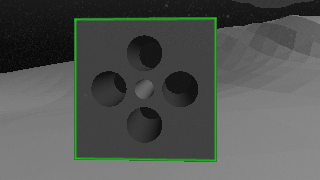
\includegraphics[width=4.5cm]{detection/clickDetLeft.png}
	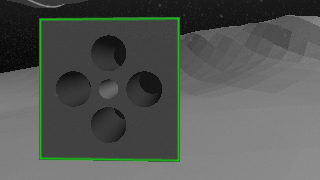
\includegraphics[width=4.5cm]{detection/clickDetRight.png}\\
	\vspace{30px}
	
	\textbf{Find Square Method}\\
	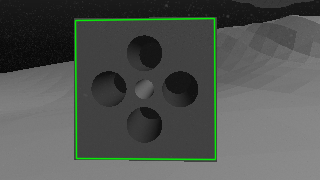
\includegraphics[width=4.5cm]{detection/squareDetLeft.png}
	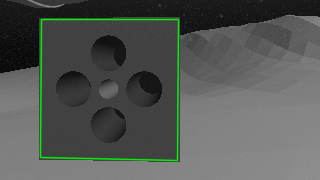
\includegraphics[width=4.5cm]{detection/squareDetRight.png}\\
	\vspace{30px}
		
	\textbf{Template Matching Method}\\
	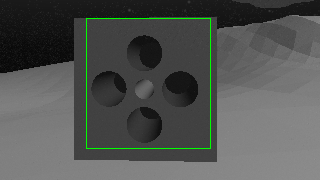
\includegraphics[width=4.5cm]{detection/tempDetLeft.png}
	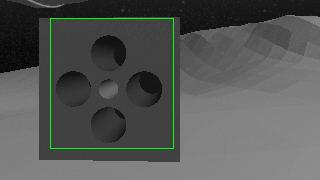
\includegraphics[width=4.5cm]{detection/tempDetRight.png}
	
	\caption[Hole Detection results with the three different methods]{Results of the three different detection method. The green rectangle is the estimate position of the square. The output of the detection step are the four corners of the green rectangle.}
	\label{fig:detectResults}
\end{figure}


\section{Tracking}
\label{sec:visTracking}
\textit{Object Tracking} means to follow the motion of an object of interest during time. Both the object and the camera can be mobile, even if, in this case, only the cameras are moving (actually, the robot moves, the cameras are rigidly attached to its body). Tracking an object is usually done to estimate its pose respect to the camera frame.\\
In this case, we speak about a \textit{markerless} \textit{model-based} tracking. Thus, the object model must be provided. In this scenario, it is sufficient to give to the algorithm the 3D dimension of the cuboid structure of the hole, with a circle in the front face. Using ViSP, the format required for the model is \textit{.cao}, which sintax is described \href{https://visp-doc.inria.fr/doxygen/visp-daily/tutorial-tracking-mb-generic.html#mb_generic_advanced_cao}{here}.\\
As explained in section \ref{sec:visDetect}, the algorithm must know the position of \textit{at least} four point belonging to the cuboid. In the experiments, the provided ones are the 4 corners of the front face.\\

Three different trackers have been tried: \textit{Two Mono Cameras Tracker} (section \ref{subsec:monoTrack}), \textit{Stereo Camera Tracker} (section \ref{subsec:stereoTrack}), and \textit{Stereo Depth Camera Tracker} (section \ref{subsec:depthTrack}).\\
A tracker is linked to each camera. For RGB cameras, it can be of three types: \textit{edge-based} [\cite{visp-edge}], \textit{keypoint-based} [\cite{visp-klt}] or a mix of both. During the experiment, the hybrid method emerged as the most precise, so all the results in section \ref{subsec:trackResult} refer to this one.
For the depth camera used in \textit{Stereo Depth Camera Tracking}, the tracker type can be \textit{normal} or \textit{dense} [\cite{visp-depth}]. Being the \textit{dense} one more robust, it is the only one to has been considered. Please note that it is also computationally heavier for large matrix computations, but speed performance are not considered here.

\subsection{Two Mono Cameras Tracking}
\label{subsec:monoTrack}
This method derived from the ViSP \textit{Markerless generic model-based tracking using a color camera} \href{https://visp-doc.inria.fr/doxygen/visp-daily/tutorial-tracking-mb-generic.html}{tutorial}.\\
The implementation is straightforward: after setting the trackers (i.e. giving edge and keypoint detection parameters, camera parameters, and 2D-3D correspondence of the four corners), at each loop the tracker estimates the transformation matrix between each camera and the object.\\
In this method, the left and right cameras are independent. Thus, each one provides a different pose estimation. It is not so easy understand when one camera provides better results that the other. Anyway, it should be easy to understand when one camera fails completely in tracking the object.

\subsection{Stereo Camera Tracking}
\label{subsec:stereoTrack}
This method derives from the ViSP \textit{Markerless generic model-based tracking using a stereo camera} \href{https://visp-doc.inria.fr/doxygen/visp-daily/tutorial-tracking-mb-generic-stereo.html}{tutorial}.\\
The code is analogous to the previous one, except that in this case also the relative pose between each camera must be provided. If this is unknown, some method for stereo calibration must be used.

\subsection{Stereo Depth Camera Tracking}
\label{subsec:depthTrack}
This method derived from the ViSP \textit{Markerless generic model-based tracking using a RGB-D camera} \href{https://visp-doc.inria.fr/doxygen/visp-daily/tutorial-tracking-mb-generic-rgbd.html}{tutorial}.\\
This method is similar to the previous one, except that the right camera is now a depth one, thus providing depth images. The functions used for depth images need the support of another library, \href{http://www.pointclouds.org/}{PCL} (Point Cloud Library) [\cite{pclLib}]. Another exception is that the depth camera does not need to initialize the 2D-3D correspondences, so the \textit{Detection} step has to be done only for the left camera.

\subsection{Tracking Results}
\label{subsec:trackResult}

In this section, performance of the three tracker are evaluated. For each one, the three different types of detection initialization (explained in \ref{sec:visDetect}) are considered to see the effect of detection error on each tracker.\\
Experiments have been conducted with lot of simplifications: no disturbance, no cameras distortions, very good visibility, nice object shape. Results described here can give only an idea on how to proceed in a more realistic scenario.\\
In the scenario, the robot is perfectly still while tracking the object, and it is in front of the object, slightly on the right. The original images taken from cameras are cut to delete a region where part of the vehicle is visible. This is done to make this part not interfere with the algorithm. In the depth image, this is not necessary, because there is no interference.\\
In fig. \ref{fig:photoTracking} the detected shape and the estimated frame are drawn on the camera images. Differences are barely visible in the first two initialization methods. With the template matching method, bad initialization (shown in \ref{subsec:detectResult}) is paid in tracking result, especially in the depth case. This is clear in fig. \ref{fig:templateErrors}. With this initialization, the depth-stereo method is even worse than the monocular case. This can be due to the fact that the depth image is not initialized with 2D-3D correspondence; thus paying more the initialization error being done only in the left image. So, it is showed that it is not always better to have a RGB-D camera instead a normal RGB. This is an interesting result and should be further explored with more realistic scenarios.\\
With good initialization, (fig. \ref{fig:clickErrors}, fig. \ref{fig:squareErrors}), the stereo methods have similar results, overall better than the mono case. which however has
not bad performance. Another interesting result is that, in the monocular case, the position of the camera influence the results. This is because different view angle obviously provides different tracking performance.\\
In the plot of the errors (fig. \ref{fig:clickErrors}, fig. \ref{fig:squareErrors}, fig. \ref{fig:templateErrors}), lot of variations during time can be seen, although the robot is still. This is due to the nature of the tracking algorithm, which continuously estimates the pose for each image received by the camera. However, it must be noticed that the variations are little for both linear and angular parts.\\

\begin{figure}[H]
	\begin{center}
		\textbf{Already known Coordinate Initialization}
	\end{center}
	\vspace{-10px}	
   	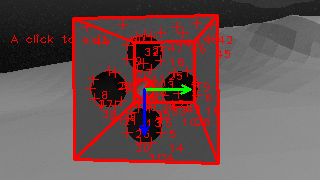
\includegraphics[width=3.4cm]{tracking/click/mono_left.png}
	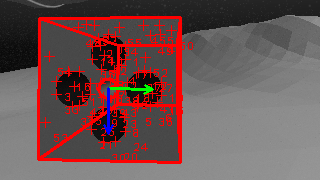
\includegraphics[width=3.4cm]{tracking/click/mono_right.png}
	\hspace{10px}
	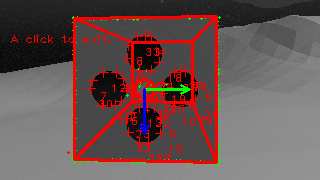
\includegraphics[width=3.4cm]{tracking/click/stereo_left.png}
	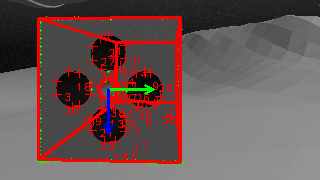
\includegraphics[width=3.4cm]{tracking/click/stereo_right.png}\\
	{\footnotesize \hspace*{20px}\textit{Mono Cameras Case} \hspace{120px} \textit{Stereo Cameras Case}}\\
	\centering{
		
	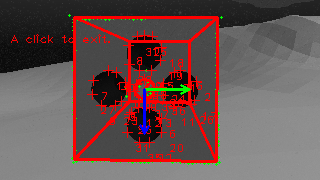
\includegraphics[width=3.4cm]{tracking/click/depth_left.png}
	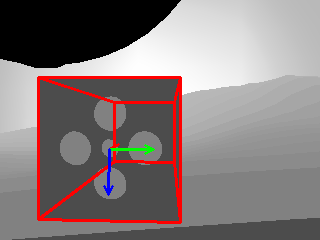
\includegraphics[width=3.4cm]{tracking/click/depth_right.png}}\\
    {\footnotesize \textit{Stereo Depth Camera Case}}\\  
\end{figure}
\vspace{-12px}
\begin{figure}[H]
	\begin{center}
		 \textbf{Find Square Initialization}
	\end{center}
	\vspace{-10px}
	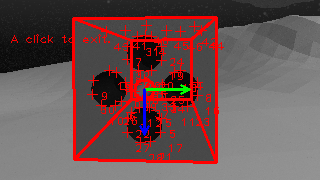
\includegraphics[width=3.4cm]{tracking/square/mono_left.png}
	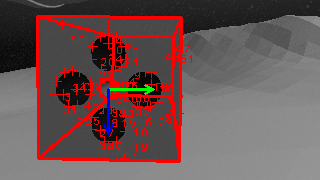
\includegraphics[width=3.4cm]{tracking/square/mono_right.png}
	\hspace{10px}
	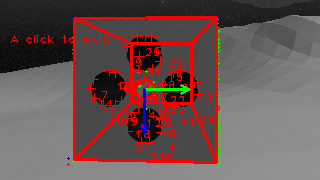
\includegraphics[width=3.4cm]{tracking/square/stereo_left.png}
	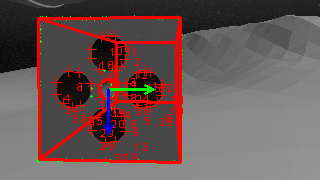
\includegraphics[width=3.4cm]{tracking/square/stereo_right.png}\\
	{\footnotesize \hspace*{20px}\textit{Mono Cameras Case} \hspace{120px} \textit{Stereo Cameras Case}}\\
	\centering{
		
	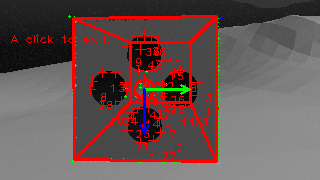
\includegraphics[width=3.4cm]{tracking/square/depth_left.png}
	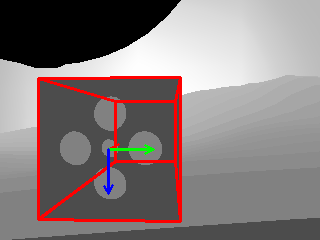
\includegraphics[width=3.4cm]{tracking/square/depth_right.png}}\\
    {\footnotesize \textit{Stereo Depth Camera Case}}\\  
\end{figure}
\vspace{-12px}
\begin{figure}[H]
	\begin{center}
		\textbf{Template Matching Initialization}
	\end{center}
	\vspace{-10px}
	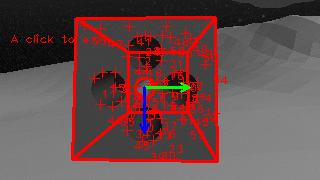
\includegraphics[width=3.4cm]{tracking/templ/mono_left.png}
	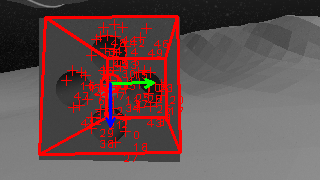
\includegraphics[width=3.4cm]{tracking/templ/mono_right.png}
	\hspace{10px}
	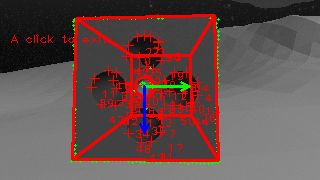
\includegraphics[width=3.4cm]{tracking/templ/stereo_left.png}
	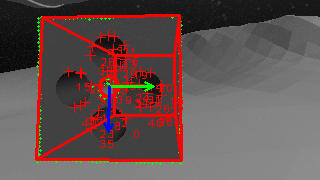
\includegraphics[width=3.4cm]{tracking/templ/stereo_right.png}\\
	{\footnotesize \hspace*{20px}\textit{Mono Cameras Case} \hspace{120px} \textit{Stereo Cameras Case}}\\
	\centering{
		
	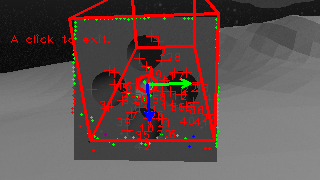
\includegraphics[width=3.4cm]{tracking/templ/depth_left.png}
	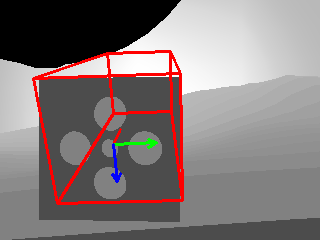
\includegraphics[width=3.4cm]{tracking/templ/depth_right.png}}\\
    {\footnotesize \textit{Stereo Depth Camera Case}}\\
\end{figure}
\captionof{figure}[Tracking Results with the three different detection initialization]{Tracking Results. Red lines are the contours of the model where is estimated to be ; red cross are the point tracked by the algorithm. The arrows represent the estimated object frame: green for y-axis, blue for z-axis, red for x-axis (which go inside the hole and is barely visible). Green dots are the tracked correspondent points between left and right images, thus they are present only in the stereo cases.}
\label{fig:photoTracking}

\begin{figure}
	\centering
	\textbf{Already known Coordinate Initialization}\\
	\vspace*{20px}
	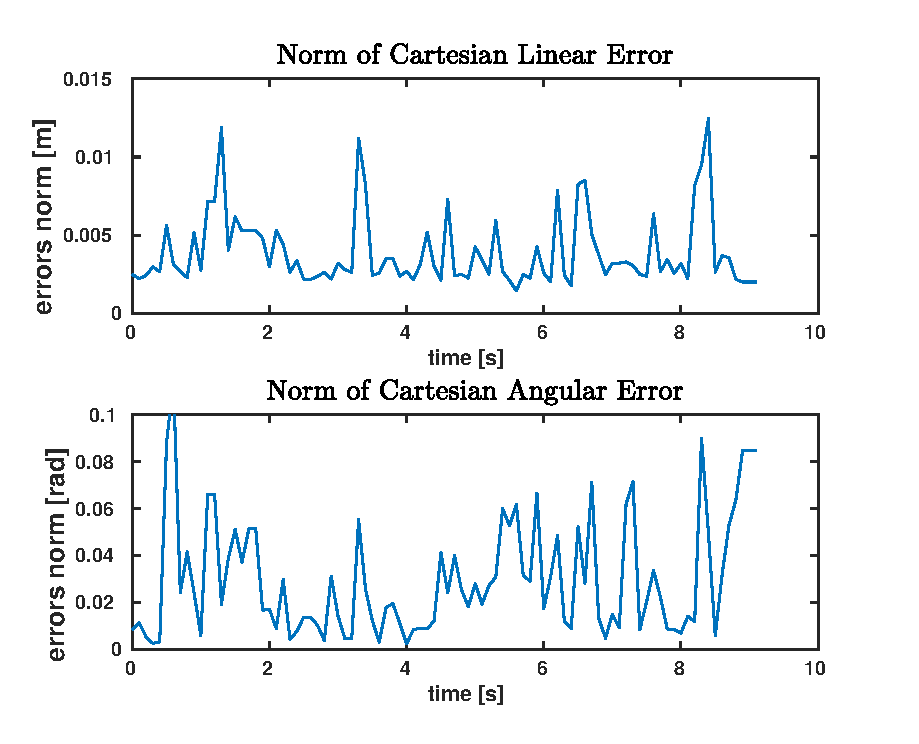
\includegraphics[width=7.15cm]{tracking/click-mono-left.eps}
	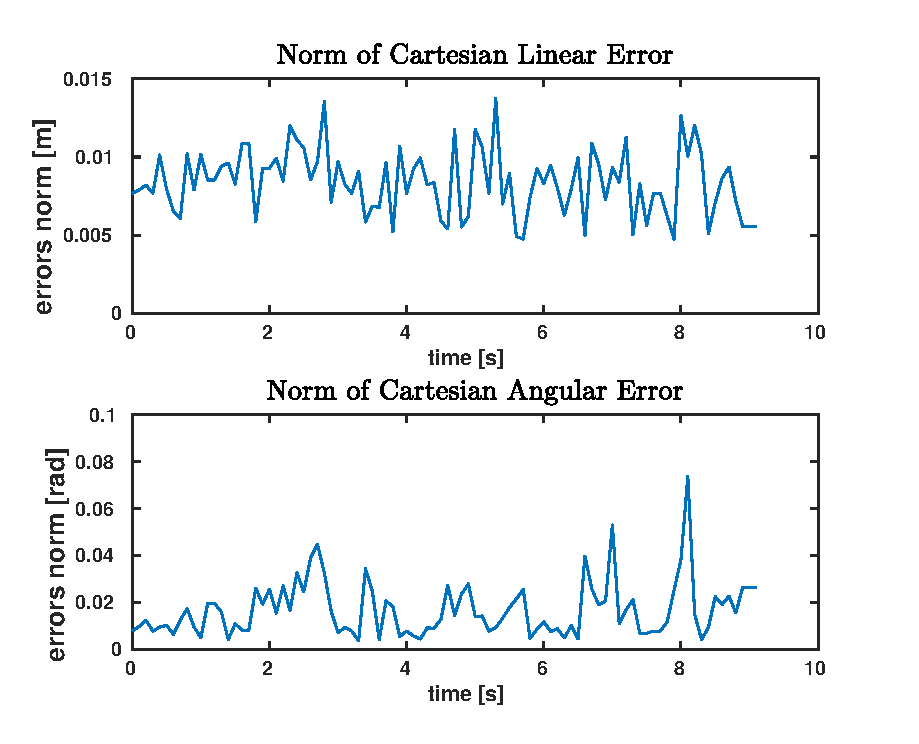
\includegraphics[width=7.15cm]{tracking/click-mono-right.eps}\\
	\hspace*{15px}\textit{Mono (left Camera) Case} \hspace{55px} \textit{Mono (right Camera) Case}\\
	\vspace{30px}
	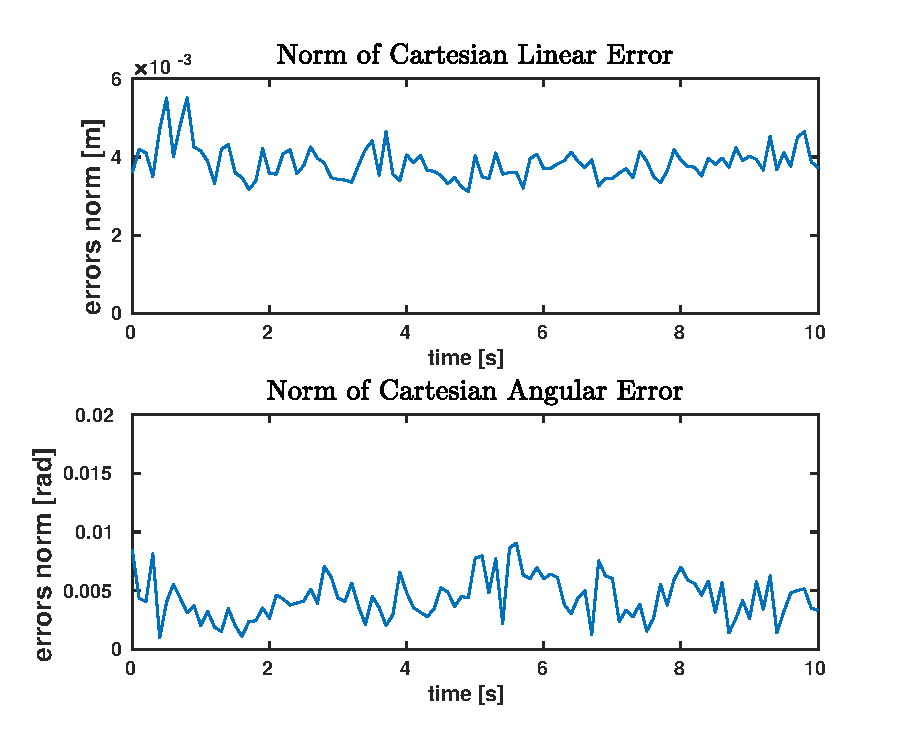
\includegraphics[width=7.15cm]{tracking/click-stereo.eps}
	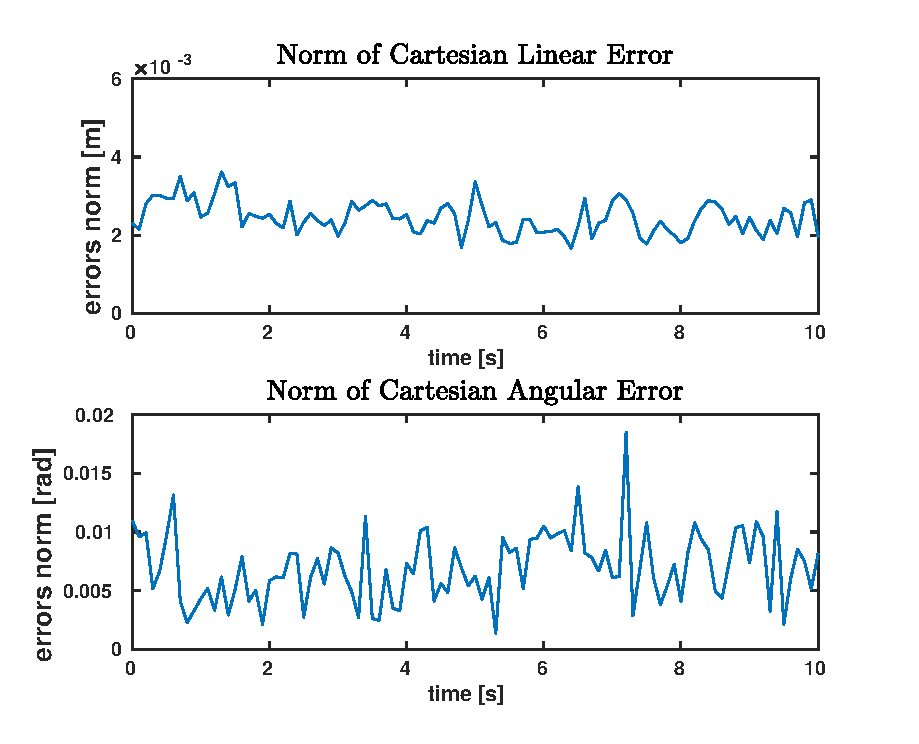
\includegraphics[width=7.15cm]{tracking/click-depth.eps}\\
	\hspace*{20px}\textit{Stereo Camera Case} \hspace{75px} \textit{Stereo Depth Camera Case}\\
	\vspace{30px}
	\caption[Tracking error plots with ideal detection initialization]{Linear and Angular Error (in norm) between true pose and estimated pose, with the best initialization of detection step possible.}
	\label{fig:clickErrors}
\end{figure}

\begin{figure}
	\centering
	\textbf{Find Square Initialization}\\
	\vspace*{20px}
	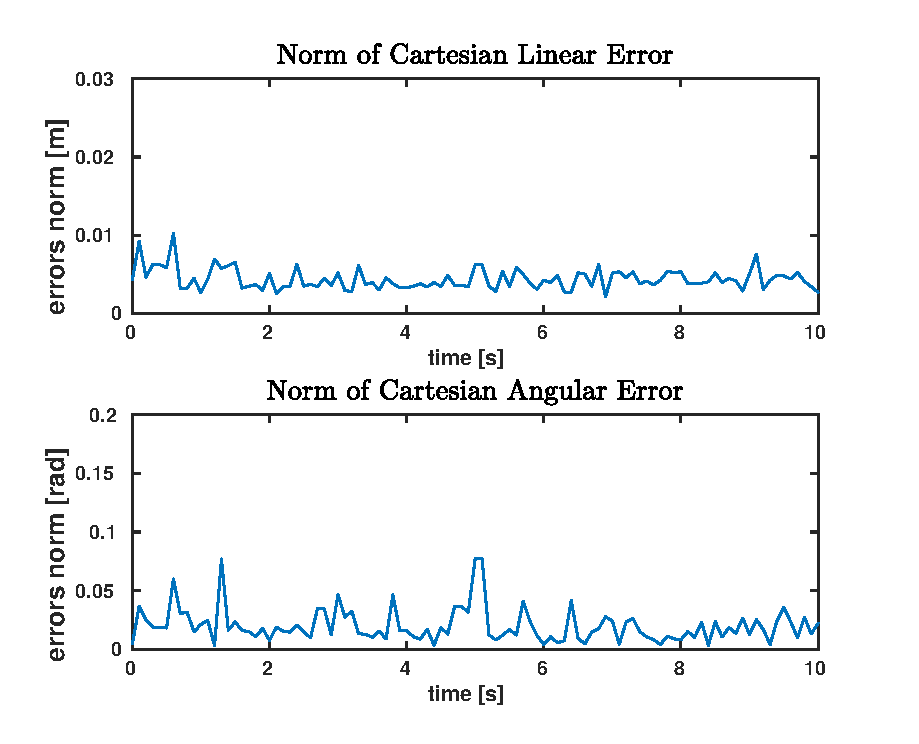
\includegraphics[width=7.15cm]{tracking/square-mono-left.eps}
	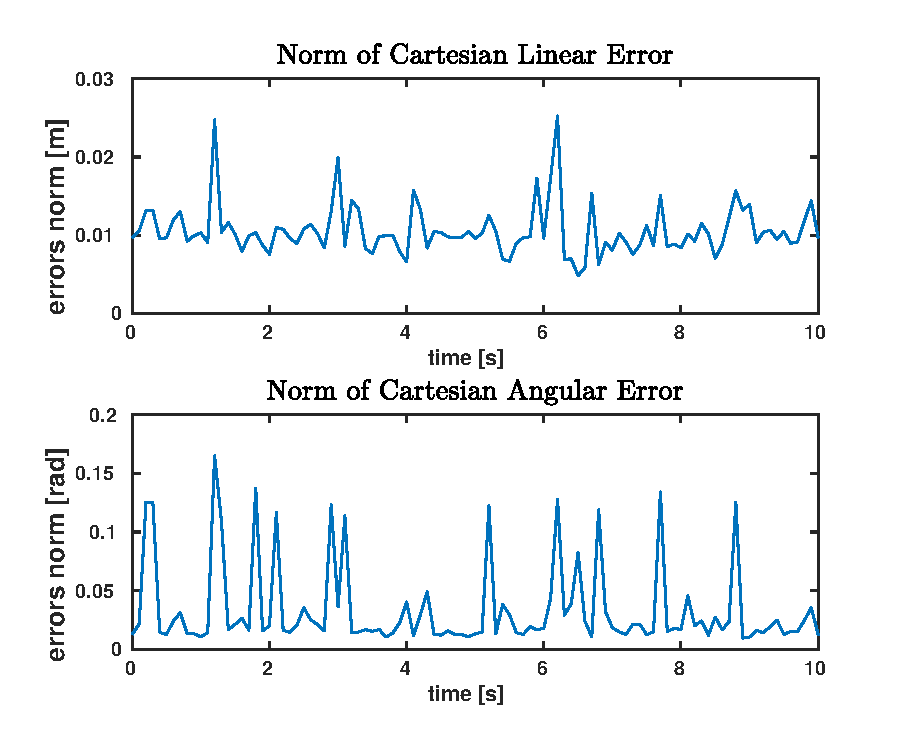
\includegraphics[width=7.15cm]{tracking/square-mono-right.eps}\\
	\hspace*{15px}\textit{Mono (left Camera) Case} \hspace{55px} \textit{Mono (right Camera) Case}\\
	\vspace{30px}
	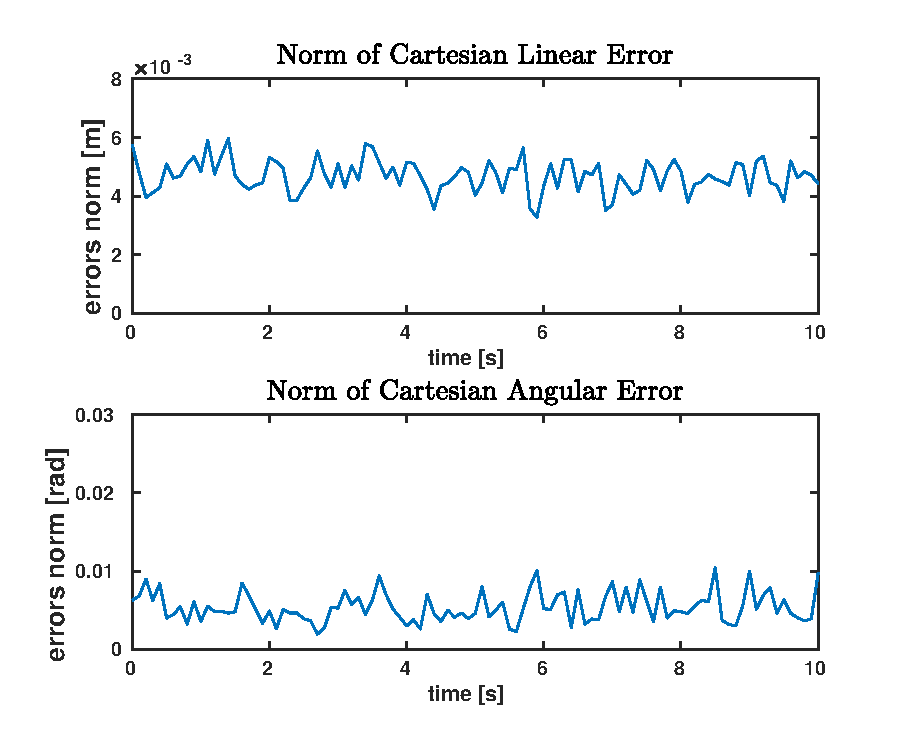
\includegraphics[width=7.15cm]{tracking/square-stereo.eps}
	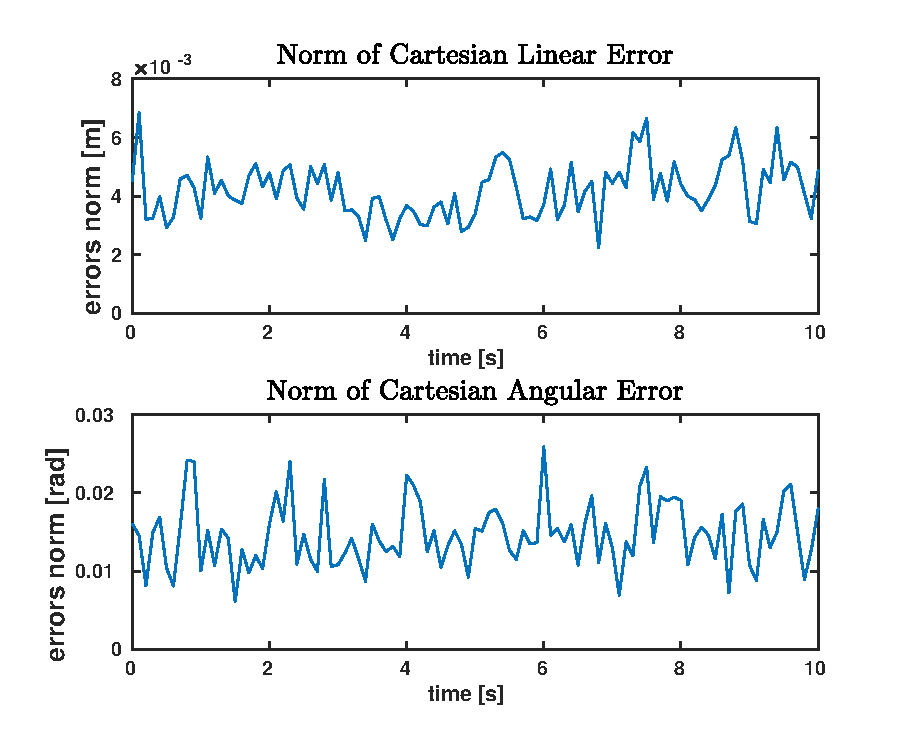
\includegraphics[width=7.15cm]{tracking/square-depth.eps}\\
	\hspace*{20px}\textit{Stereo Camera Case} \hspace{75px} \textit{Stereo Depth Camera Case}\\
	\vspace{30px}
	\caption[Tracking error plots with find square detection initialization]{Linear and Angular Error (in norm) between true pose and estimated pose. The detection step here used the find square method.}
	\label{fig:squareErrors}
\end{figure}

\begin{figure}
	\centering
	\textbf{Template Matching Initialization}\\
	\vspace*{20px}
	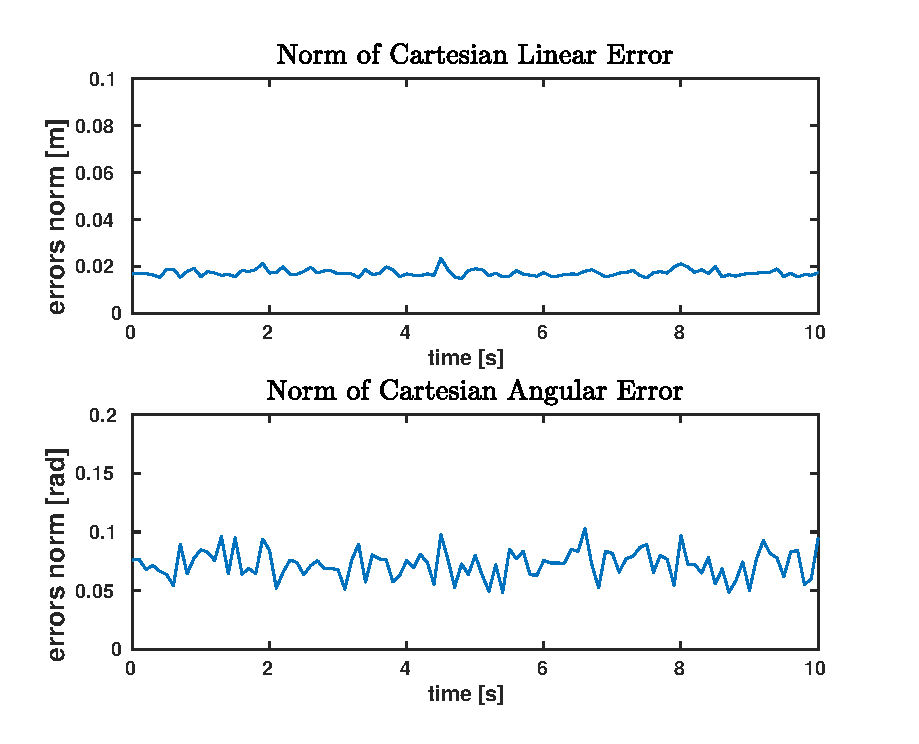
\includegraphics[width=7.15cm]{tracking/templ-mono-left.eps}
	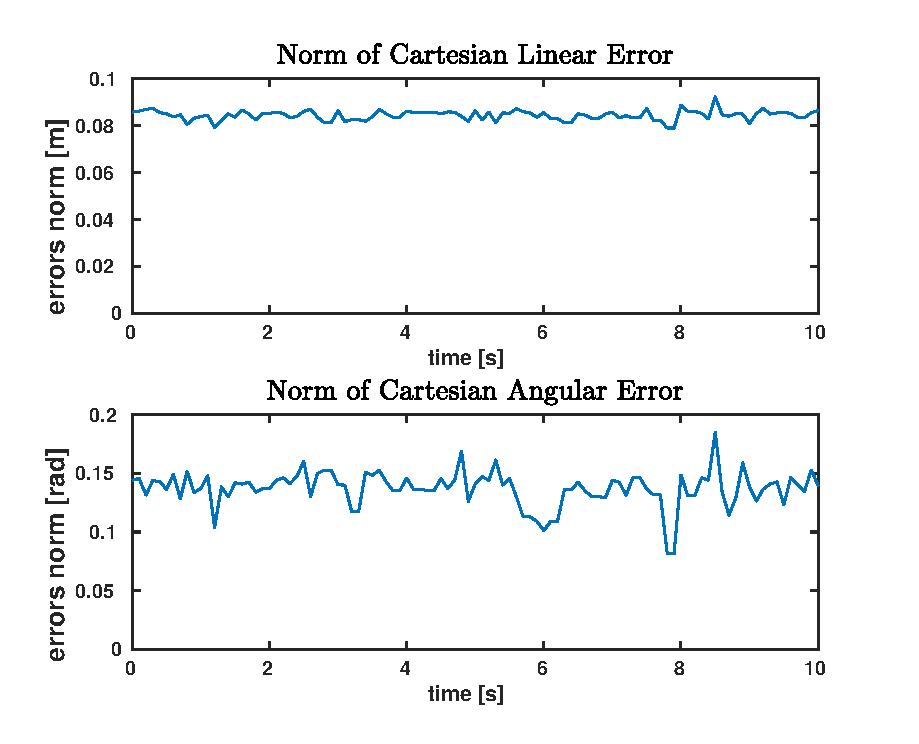
\includegraphics[width=7.15cm]{tracking/templ-mono-right.eps}\\
	\hspace*{15px}\textit{Mono (left Camera) Case} \hspace{55px} \textit{Mono (right Camera) Case}\\
	\vspace{30px}
	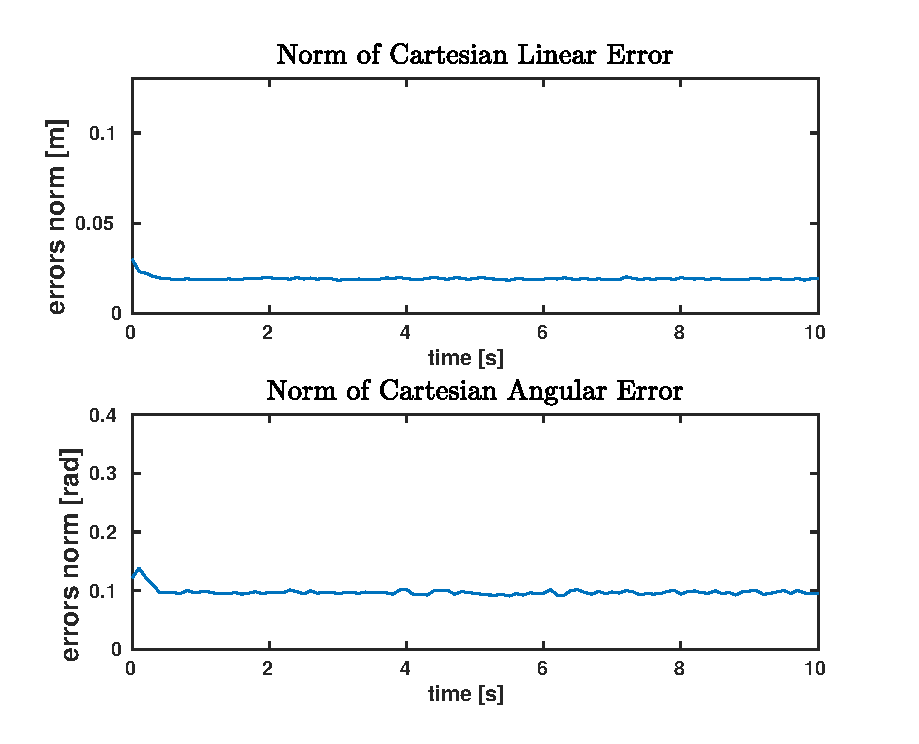
\includegraphics[width=7.15cm]{tracking/templ-stereo.eps}
	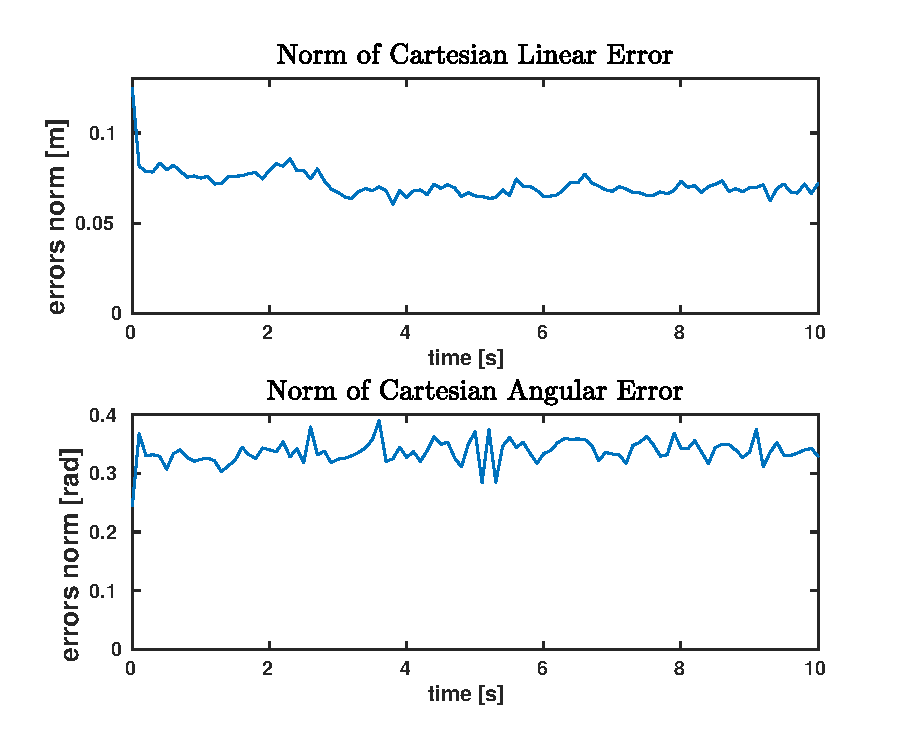
\includegraphics[width=7.15cm]{tracking/templ-depth.eps}\\
	\hspace*{20px}\textit{Stereo Camera Case} \hspace{75px} \textit{Stereo Depth Camera Case}\\
	\vspace{30px}
	\caption[Tracking error plots with template matching detection initialization]{Linear and Angular Error (in norm) between true pose and estimated pose. The detection step here used the template matching method.}
	\label{fig:templateErrors}
\end{figure}